\documentclass[c]{beamer}  % [t], [c], или [b] --- вертикальное выравнивание на слайдах (верх, центр, низ)

\usetheme{Singapore}
\usecolortheme{rose}


\usepackage[rightcaption]{sidecap}
\usepackage[russian]{babel}
\usepackage{hyperref}
\usepackage[usenames,dvipsnames,svgnames,table,rgb]{xcolor}
\hypersetup{				% Гиперссылки
    unicode=true,           % русские буквы в раздела PDF
    colorlinks=true,       	% false: ссылки в рамках; true: цветные ссылки
    linkcolor=violet,          % внутренние ссылки
    citecolor=green,        % на библиографию
    filecolor=magenta,      % на файлы
    urlcolor=pink          % на URL
}

%% Created with wxMaxima 23.05.1

\setlength{\parskip}{\medskipamount}
\setlength{\parindent}{0pt}
\usepackage{iftex}
\ifPDFTeX
  % PDFLaTeX or LaTeX 
  \usepackage[utf8]{inputenc}
  \usepackage[T1]{fontenc}
  \DeclareUnicodeCharacter{00B5}{\ensuremath{\mu}}
\else
  %  XeLaTeX or LuaLaTeX
  \usepackage{fontspec}
\fi
\usepackage{graphicx}
\usepackage{color}
\usepackage{amsmath}
\usepackage{grffile}
\usepackage{ifthen}
\newsavebox{\picturebox}
\newlength{\pictureboxwidth}
\newlength{\pictureboxheight}
\newcommand{\includeimage}[1]{
    \savebox{\picturebox}{\includegraphics{#1}}
    \settoheight{\pictureboxheight}{\usebox{\picturebox}}
    \settowidth{\pictureboxwidth}{\usebox{\picturebox}}
    \ifthenelse{\lengthtest{\pictureboxwidth > .95\linewidth}}
    {
        \includegraphics[width=.55\linewidth,height=.40\textheight,keepaspectratio]{#1}
    }
    {
        \ifthenelse{\lengthtest{\pictureboxheight>.80\textheight}}
        {
            \includegraphics[width=.55\linewidth,height=.40\textheight,keepaspectratio]{#1}
            
        }
        {
            \includegraphics{#1}
        }
    }
}
\newlength{\thislabelwidth}
\DeclareMathOperator{\abs}{abs}

\definecolor{labelcolor}{RGB}{100,0,0}
% \setlength{\topmargin}{-0.5in}
% \setlength{\oddsidemargin}{0 in}
% \textwidth 160mm
% \textheight 220mm
\title{Экстремальные задачи на графах}
\author{Рузанова Дарья\\ ММБ-102}
\institute[ОмГУ]{Омский государственный университет \\ им. Ф.М. Достоевского}
\date{Омск 2024}
\begin{document}

\frame{\titlepage}

\begin{frame}{Задание 1}

% \singlespacing % Reset line spacing to 1 from here on


Граф $G$ и выделенное в нем остовное дерево:\\

\[
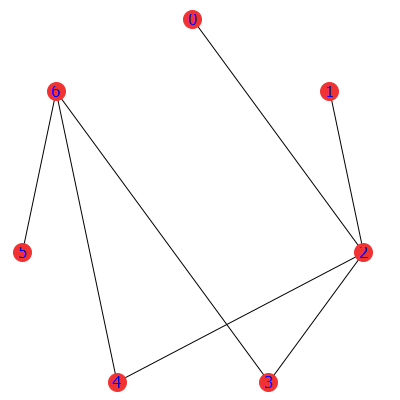
\includegraphics[width=.55\linewidth,height=.40\textheight,keepaspectratio]{graphs_img/graphs_1}
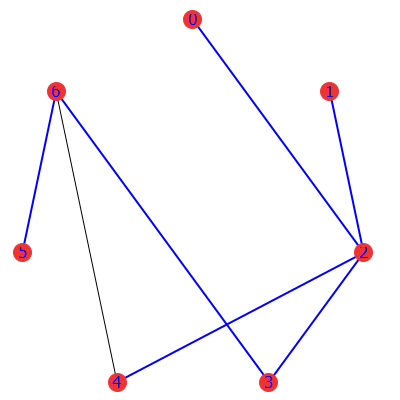
\includegraphics[width=.55\linewidth,height=.40\textheight,keepaspectratio]{graphs_img/graphs_3}\]

\end{frame}
\begin{frame}
\frametitle{Задание 1}
Минимальное множество сочленений графа и минимальный разрез:

\[\displaystyle 
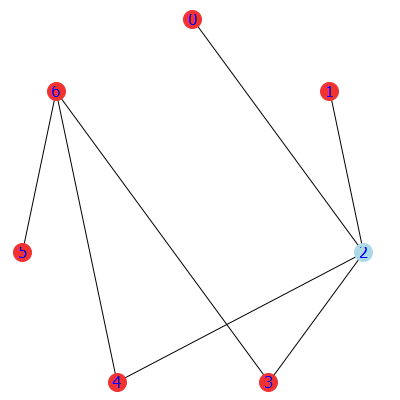
\includegraphics[width=.55\linewidth,height=.40\textheight,keepaspectratio]{graphs_img/graphs_4}
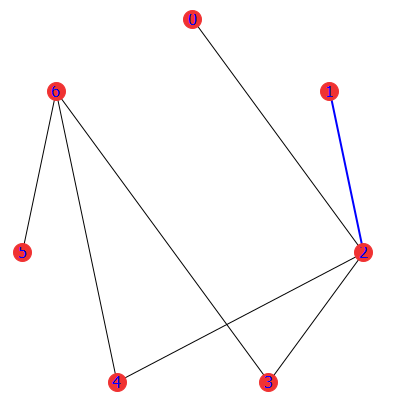
\includegraphics[width=.55\linewidth,height=.40\textheight,keepaspectratio]{graphs_img/graphs_5}\]

\end{frame}
\begin{frame}
\frametitle{Задание 1}
Выделим блоки графа $G$:\\
\[\displaystyle
\left[ \left[ 5\operatorname{,}6\right] \operatorname{,}\left[ 1\operatorname{,}2\right] \operatorname{,}\left[ 0\operatorname{,}2\right] \operatorname{,
}\]\[\left[ 2\operatorname{,}3\operatorname{,}4\operatorname{,}6\right] \right] \mbox{}
\]
%%%%%%%%%%%%%%%%
\end{frame}
\begin{frame}
\frametitle{Задание 1}


Минимальное вершинное покрытие и максимальное
независимое множество вершин:\\
\[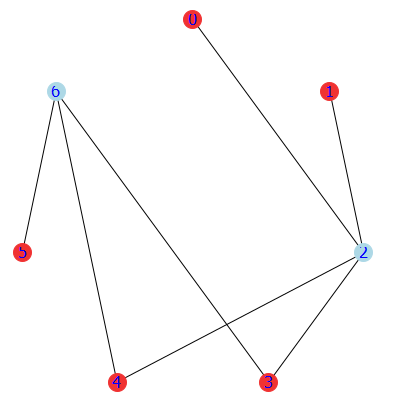
\includegraphics[width=.55\linewidth,height=.40\textheight,keepaspectratio]{graphs_img/graphs_6}
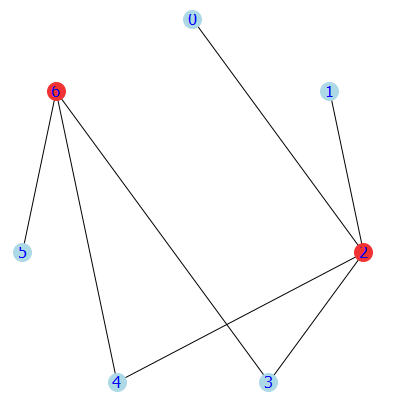
\includegraphics[width=.55\linewidth,height=.40\textheight,keepaspectratio]{graphs_img/graphs_7}\mbox{}\]

\end{frame}
\begin{frame}
\frametitle{Задание 1}
Максимальная клика графа $G$:

\[\displaystyle
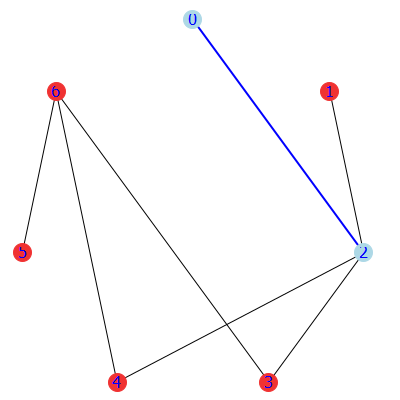
\includegraphics[width=.75\linewidth,height=.60\textheight,keepaspectratio]{graphs_img/graphs_8}\mbox{}\]

\end{frame}
\begin{frame}{Задание 2}
Граф $S$ с выделенным максимальным паросочетанием:

\[ 
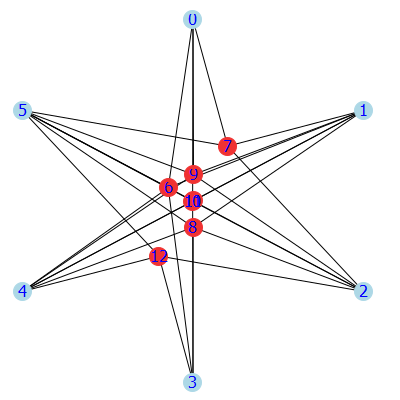
\includegraphics[width=.65\linewidth,height=.50\textheight,keepaspectratio]{graphs_img/graphs_9}\mbox{}\]

Найденное паросочетание не является совершенным, потому что не покрывает вершину с номером $6$.
\end{frame}
\begin{frame}{Задание 3}
Взвешенный граф $G_{copy}$, на котором выделен кратчайший путь:\\
\[\displaystyle 
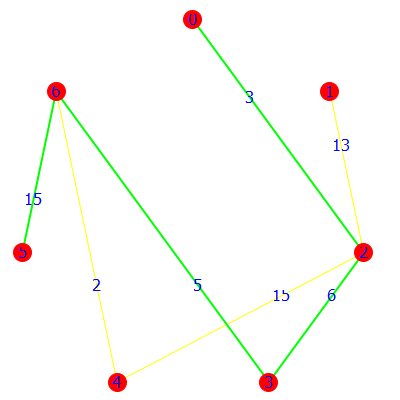
\includegraphics[width=.65\linewidth,height=.50\textheight,keepaspectratio]{graphs_img/graphs_11}\mbox{}\]
Длина кратчайшего пути: 29.
\end{frame}
\begin{frame}{Задание 4}
Сеть G4:\\

\[\displaystyle 
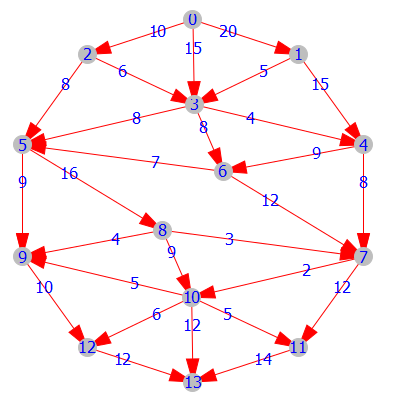
\includegraphics[width=.75\linewidth,height=.60\textheight,keepaspectratio]{graphs_img/graphs_12}\mbox{}\]
\end{frame}
\begin{frame}
\frametitle{Задание 4}
%%%%%%%%%%%%%%%%

Максимальный поток в сети $G4$ и его распределение по дугам:\\

%%%% OUTPUT:
\[\displaystyle
\operatorname{[}33\operatorname{,}\operatorname{[}\left[ \left[ 0\operatorname{,}1\right] \operatorname{,}15\right] \operatorname{,}\left[ \left[ 0\operatorname{,}3\right] \operatorname{,}14\right] \operatorname{,}\left[ \left[ 0\operatorname{,}2\right] \operatorname{,}4\right] \operatorname{,}\left[ \left[ 1\operatorname{,}4\right] \operatorname{,}15\right] \operatorname{,
}\left[ \left[ 1\operatorname{,}3\right] \operatorname{,}0\right] \operatorname{,}\]\[\left[ \left[ 2\operatorname{,}3\right] \operatorname{,}0\right] \operatorname{,}\left[ \left[ 2\operatorname{,}5\right] \operatorname{,}4\right] \operatorname{,}\left[ \left[ 3\operatorname{,}4\right] \operatorname{,}0\right] \operatorname{,}\left[ \left[ 3\operatorname{,}6\right] \operatorname{,}6\right] \operatorname{,}\left[ \left[ 3\operatorname{,}5\right] \operatorname{,}8\right] \operatorname{,
}\left[ \left[ 4\operatorname{,}6\right] \operatorname{,}7\right] \operatorname{,}\left[ \left[ 4\operatorname{,}7\right] \operatorname{,}\]
\[8\right] \operatorname{,}\left[ \left[ 5\operatorname{,}8\right] \operatorname{,}10\right] \operatorname{,}\left[ \left[ 5\operatorname{,}9\right] \operatorname{,}9\right] \operatorname{,}\left[ \left[ 6\operatorname{,}5\right] \operatorname{,}7\right] \operatorname{,}\left[ \left[ 6\operatorname{,}7\right] \operatorname{,}6\right] \operatorname{,
}\left[ \left[ 7\operatorname{,}11\right] \operatorname{,}12\right] \operatorname{,}\left[ \left[ 7\operatorname{,}10\right] \operatorname{,}2\right] \operatorname{,}\left[ \left[ 8\operatorname{,}7\right] \operatorname{,}0\right] \operatorname{,}\left[ \left[ 8\operatorname{,}10\right] \operatorname{,}9\right] \operatorname{,}\left[ \left[ 8\operatorname{,}9\right] \operatorname{,}1\right] \operatorname{,
}\left[ \left[ 9\operatorname{,}12\right] \operatorname{,}\]\[10\right] \operatorname{,}\left[ \left[ 10\operatorname{,}9\right] \operatorname{,}0\right] \operatorname{,}\left[ \left[ 10\operatorname{,}11\right] \operatorname{,}0\right] \operatorname{,}\left[ \left[ 10\operatorname{,}13\right] \operatorname{,}11\right] \operatorname{,}\left[ \left[ 10\operatorname{,}12\right] \operatorname{,}0\right] \operatorname{,
}\left[ \left[ 11\operatorname{,}13\right] \operatorname{,}12\right] \operatorname{,}\left[ \left[ 12\operatorname{,}13\right] \operatorname{,}10\right] \operatorname{]}\operatorname{]}\mbox{}
\]
%%%%%%%%%%%%%%%%
\end{frame}
\begin{frame}{Заключение}
\begin{block}{Цель исследования:} C помощью специализированного пакета $graphs$, создать обычный граф, случайный двудольный граф, взвешенный и сеть. Изучить их свойства и построить изображения графов, выделив определенные его элементы.

\end{block}
\begin{block}{Использованные средства:} Исследование производилось с помощью программы wxMaxima.\\
\end{block}
\end{frame}

\begin{frame}
\frametitle{Заключение}
\begin{block}{Результат:} 
\begin{itemize}
\footnotesize
    \item В графе $G$ было найдено остовное дерево, минимальное множество сочленения, минимальный разрез, минимальное вершинное покрытие, максимальное независимое множество вершин, найдена клика и были выделены его блоки.

\end{itemize}	
\end{block}
 \end{frame}

\begin{frame}
\frametitle{Заключение}
\begin{block}{Результат:} 
\begin{itemize}
\footnotesize
    \item В графе $G$ было найдено остовное дерево, минимальное множество сочленения, минимальный разрез, минимальное вершинное покрытие, максимальное независимое множество вершин, найдена клика и были выделены его блоки.

    \item Для случайного двудольного графа $S$ было найдено его максимальное паросочетание графа.

\end{itemize}	
\end{block}
 \end{frame}


 \begin{frame}
\frametitle{Заключение}
\begin{block}{Результат:} 
\begin{itemize}
\footnotesize
    \item В графе $G$ было найдено остовное дерево, минимальное множество сочленения, минимальный разрез, минимальное вершинное покрытие, максимальное независимое множество вершин, найдена клика и были выделены его блоки.

    \item Для случайного двудольного графа $S$ было найдено его максимальное паросочетание графа.

    \item В взвешенном графе $G_{copy}$ был найден кратчайший путь из вершины с номером $0$ в вершину с номером $5$ и найдена его длина.

\end{itemize}	
\end{block}
 \end{frame}

 \begin{frame}
\frametitle{Заключение}
\begin{block}{Результат:} 
\begin{itemize}
\footnotesize
    \item В графе $G$ было найдено остовное дерево, минимальное множество сочленения, минимальный разрез, минимальное вершинное покрытие, максимальное независимое множество вершин, найдена клика и были выделены его блоки.

    \item Для случайного двудольного графа $S$ было найдено его максимальное паросочетание графа.

    \item В взвешенном графе $G_{copy}$ был найден кратчайший путь из вершины с номером $0$ в вершину с номером $5$ и найдена его длина.

    \item В данной сети $G4$ был найден максимальный поток в сети и его распределение по дугам.

\end{itemize}	
\end{block}
 \end{frame}
 \begin{frame}
\frametitle{Заключение}
 \begin{block}{Результат:} 
\begin{itemize}
\footnotesize
    \item В графе $G$ было найдено остовное дерево, минимальное множество сочленения, минимальный разрез, минимальное вершинное покрытие, максимальное независимое множество вершин, найдена клика и были выделены его блоки.

    \item Для случайного двудольного графа $S$ было найдено его максимальное паросочетание графа.

    \item В взвешенном графе $G_{copy}$ был найден кратчайший путь из вершины с номером $0$ в вершину с номером $5$ и найдена его длина.

    \item В данной сети $G4$ был найден максимальный поток в сети и его распределение по дугам.

    \item Для всех графов были построены соответствующие изображения.
\end{itemize}	
\end{block}
 \end{frame}
 
\end{document}
